\documentclass[12pt,letterpaper]{exam}
\usepackage[lmargin=1in,rmargin=1in,tmargin=1in,bmargin=1in]{geometry}
\usepackage{../style/exams}

% -------------------
% Course & Exam Information
% -------------------
\newcommand{\course}{MATH 141: Exam 2}
\newcommand{\term}{Spring --- 2025}
\newcommand{\examdate}{03/07/2025}
\newcommand{\timelimit}{50 Minutes}

\setbool{hideans}{false} % Student: True; Instructor: False

\newcommand{\lh}{\stackrel{\text{L.H.}}{=}}

% -------------------
% Content
% -------------------
\begin{document}

\examtitle
\instructions{Write your name on the appropriate line on the exam cover sheet. This exam contains \numpages\ pages (including this cover page) and \numquestions\ questions. Check that you have every page of the exam. Answer the questions in the spaces provided on the question sheets. Be sure to answer every part of each question and show all your work. If you run out of room for an answer, continue on the back of the page --- being sure to indicate the problem number.} 
\scores
\bottomline
\newpage


% -------------------
% Questions
% -------------------
\begin{questions}

% Question 1
\newpage
\question[20] Let $f(x)$ be a twice continuously differentiable function whose \textit{derivative}, $f'(x)$, is plotted below.
	\[
	\fbox{
	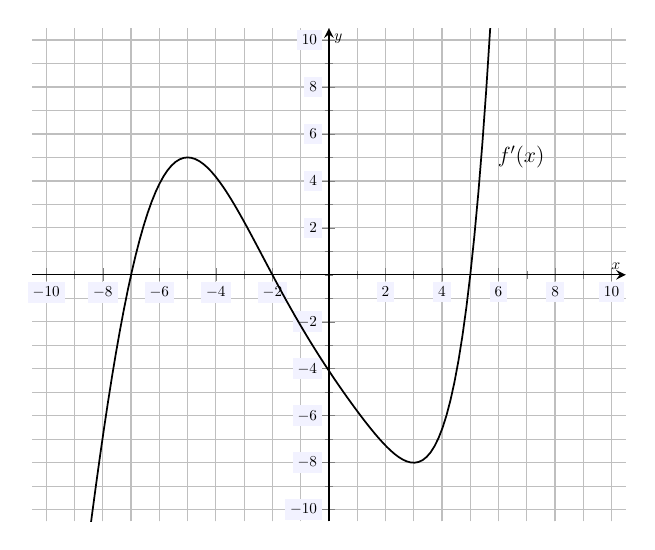
\begin{tikzpicture}[scale=1.1,every node/.style={scale=0.5}]
	\begin{axis}[
	grid=both,
	axis lines=middle,
	ticklabel style={fill=blue!5!white},
	xmin= -10.5, xmax=10.5,
	ymin= -10.5, ymax=10.5,
	xtick={-10,-8,-6,-4,-2,0,2,4,6,8,10},
	ytick={-10,-8,-6,-4,-2,0,2,4,6,8,10},
	minor tick = {-10,-9,...,10},
	xlabel=\(x\),ylabel=\(y\),
	]
	\addplot[line width= 0.02cm,samples=150,domain= -10.5:10.5] ({x},{-4.08789 - 1.80944*x + 0.102687*x^2 - 0.0121406*x^3 + 0.00202778*x^4 + 0.00258073*x^5 + 0.000176215*x^6});
	\node at (6.8,5) {\Large$f'(x)$};
	\end{axis}
	\end{tikzpicture}
	}
	\] 
Based on the plot above, answer the following questions: 
	\begin{enumerate}[(a)]
	\item On what interval(s)---if any---is $f(x)$ increasing? \vfill
	
	{\itshape\small If $f'(x) > 0$, then $f(x)$ is increasing. Therefore, $f(x)$ is increasing on $(-7, -2) \cup (5, \infty)$.}  \vfill
	
	\item On what interval(s)---if any---is $f(x)$ decreasing? \vfill
	
	{\itshape\small If $f'(x) < 0$, then $f(x)$ is decreasing. Therefore, $f(x)$ is decreasing on $(-\infty, -7) \cup (-2, 5)$.} \vfill
	
	\item On what interval(s)---if any---is $f(x)$ concave up? \vfill
	
	{\itshape\small If $f(x)$ is concave up, then $f''(x) > 0$ so that $f'(x)$ is increasing. Therefore, $f(x)$ is concave up on $(-\infty, -5) \cup (3, \infty)$.} \vfill
	
	\item On what interval(s)---if any---is $f(x)$ concave down? \vfill
	
	{\itshape\small If $f(x)$ is concave up, then $f''(x) > 0$ so that $f'(x)$ is increasing. Therefore, $f(x)$ is concave up on $(-5, 3)$.} \vfill
	
	\item Find any critical values for $f(x)$---if any. \vfill
	
	{\itshape\small If $f(x)$ has a critical value, then $f'(x)= 0$ or is undefined. We see the critical values are $x= -7, -2, 5$.} \vfill
		
	\item Classify any critical values you found in (e). If there were none, state so. \vfill
	
	\phantom{.} \hfill 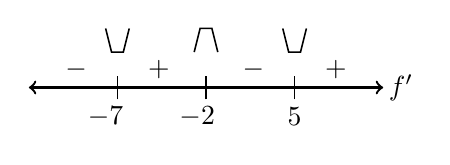
\begin{tikzpicture}[scale=0.75]
	\draw[line width=0.03cm,<->] (-3,0) -- (3,0);
	\draw[line width=0.02cm] (-1.5,-0.2) -- (-1.5,0.2);
	\draw[line width=0.02cm] (0,-0.2) -- (0,0.2);
	\draw[line width=0.02cm] (1.5,-0.2) -- (1.5,0.2);
	\node at (3.3,0) {$f'$};
	\node at (-1.7,-0.5) {$-7$};
	\node at (-0.15,-0.5) {$-2$};
	\node at (1.5,-0.5) {$5$};
	
	\node at (-2.2,0.3) {$-$};
	\node at (-0.8,0.3) {$+$};
	\node at (0.8,0.3) {$-$};
	\node at (2.2,0.3) {$+$};
	
	\draw[line width=0.02cm] (-1.7,1) -- (-1.6,0.6) -- (-1.4,0.6) -- (-1.3,1);
	\draw[line width=0.02cm] (1.3,1) -- (1.4,0.6) -- (1.6,0.6) -- (1.7,1);
	
	
	\draw[line width=0.02cm] (-0.2,0.6) -- (-0.1,1) -- (0.1,1) -- (0.2,0.6);

	
	

	\end{tikzpicture} \hfill \phantom{.}
	
	{\itshape\small Alternatively, we know $f''(x) > 0$ at $x= -7, 5$ and $f''(x) < 0$ at $x= -2$. Therefore, $x= -7, 5$ are minima and $x= 5$ is a maxima.}
	
	\item Find the $x$-value(s) for any point(s) of inflection for $f(x)$. \vfill

	{\itshape\small An inflection point is where $f''(x)$ changes sign. From (c) and (d), we can see this is at $x= -5, 3$.} \vfill 
	\end{enumerate}



% Question 2
\newpage
\question[16] Showing all your work, compute the following limits: \par\vspace{0.3cm}
	\begin{enumerate}[(a)]
	\item $\ds\lim_{x \to \infty} \left[ \ln(9x - 7) - \ln(3x + 5) \right]=$  \vfill
		\[
		\hspace{-1.5cm} \lim_{x \to \infty} \left[ \ln(9x - 7) - \ln(3x + 5) \right]= \lim_{x \to \infty} \ln \left( \dfrac{9x - 7}{3x + 5} \right)= \ln \left( \lim_{x \to \infty} \dfrac{9x - 7}{3x + 5} \right) \lh \ln \left( \lim_{x \to \infty} \dfrac{9}{3} \right)= \ln(3)
		\] \vfill\vspace{0.1cm}
	
	\item $\ds\lim_{x \to \infty} \dfrac{3 \ln(4x - 2)}{5 \ln(6x + 1)}=$  \vfill
		\[
		\lim_{x \to \infty} \dfrac{3 \ln(4x - 2)}{5 \ln(6x + 1)} \lh \lim_{x \to \infty} \dfrac{3 \cdot \dfrac{1}{4x - 2} \cdot 4}{5 \cdot \dfrac{1}{6x + 1} \cdot 6}= \lim_{x \to \infty} \dfrac{12 (6x + 1)}{30(4x - 2)} \lh \lim_{x \to \infty} \dfrac{12 \cdot 6}{30 \cdot 4}= \dfrac{3}{5}
		\] \vfill
	
	\newpage
	
	\phantom{} \par
	\item $\ds\lim_{x \to 0} \dfrac{x + \sin x}{\tan(5x)}=$  \par\vspace{2.25cm}
		\[
		\lim_{x \to 0} \dfrac{x + \sin x}{\tan(5x)} \lh \lim_{x \to 0} \dfrac{1 + \cos x}{\sec^2(5x) \cdot 5}= \dfrac{1 + \cos(0)}{\sec^2(0) \cdot 5}= \dfrac{1 + 1}{1^2  \cdot 5}= \dfrac{2}{5}
		\] \par\vspace{2.25cm}
	
	\item $\ds\lim_{x \to 0} (\cos x)^{2/x^2}$ \pspace
		\[
		\begin{aligned}
		L&:= \lim_{x \to 0} (\cos x)^{2/x^2} \\[0.2cm]
		\ln L&= \lim_{x \to 0} \ln(\cos x)^{2/x^2} \\[0.2cm]
		\ln L&= \lim_{x \to 0} \dfrac{2}{x^2} \cdot \ln(\cos x) \\[0.2cm]
		\ln L&= \lim_{x \to 0} \dfrac{2 \ln(\cos x)}{x^2} \\[0.1cm]
		\ln L&\lh \lim_{x \to 0} \dfrac{2 \cdot \left( \dfrac{1}{\cos x} \cdot -\sin x \right)}{2x} \\[0.2cm]
		\ln L&= \lim_{x \to 0} \dfrac{-\sin x}{x \cos x} \\[0.2cm]
		\ln L&\lh \lim_{x \to 0} \dfrac{-\cos x}{\cos x - x \sin x} \\[0.2cm]
		\ln L&= \dfrac{-\cos(0)}{\cos(0) - 0 (\sin 0)} \\[0.2cm]
		\ln L&= \dfrac{-1}{1 - 0} \\[0.2cm]
		\ln L&= \dfrac{-1}{1} \\[0.2cm]
		\ln L&= -1 \\[0.2cm]
		L&= e^{-1}
		\end{aligned}
		\]	
	\end{enumerate}



% Question 3
\newpage
\question[16] Find the area of the largest rectangle that has its `upper' vertices on the line $y= 19$ and its `lower' vertices on the function $f(x)= 2x^2 + 1$. \pspace

{\itshape\textbf{Solution.} We know the graph of $y= 19$ is a horizontal line and that the graph of $f(x)= 2x^2 + 1$ is a parabola with $y$-intercept $1$ that opens upwards. Two of the vertices are on the line. If the vertices on the parabola did not have the same $x$-coordinates as those on the line, then the vertical sides would be `slanted' and not parallel. If the $y$-coordinates of the vertices on the parabola were not the same, the horizontal sides would not be parallel. Finally, $f(a)= f(b)$ if and only if $a= \pm b$. Therefore, the rectangle is as shown below.
	\[
	\fbox{
	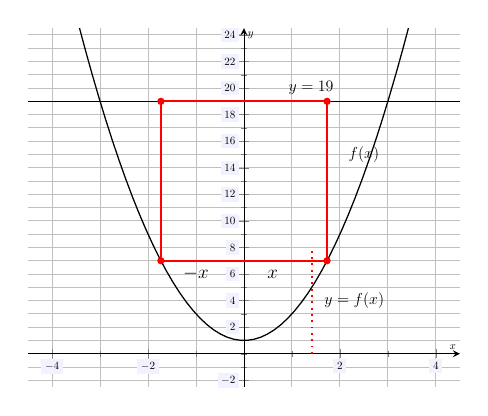
\begin{tikzpicture}[scale=0.8,every node/.style={scale=0.5}]
	\begin{axis}[
	grid=both,
	axis lines=middle,
	ticklabel style={fill=blue!5!white},
	xmin= -4.5, xmax=4.5,
	ymin= -2.5, ymax=24.5,
	xtick={-4,-2,...,4},
	ytick={-6,-4,...,26},
	minor tick = {-25,-24,...,25},
	xlabel=\(x\),ylabel=\(y\),
	]
	\addplot[line width= 0.02cm,samples=150,domain= -10.5:10.5] ({x},{19});
	\addplot[line width= 0.02cm,samples=150,domain= -10.5:10.5] ({x},{2*x^2 + 1});
	\node at (2.5,15) {\Large$f(x)$};
	
	\node[circle,fill=red,minimum size=0.04cm,scale=0.7] at (-1.73205,19) {};
	\node[circle,fill=red,minimum size=0.04cm,scale=0.7] at (-1.73205,7) {};
	\node[circle,fill=red,minimum size=0.04cm,scale=0.7] at (1.73205,7) {};
	\node[circle,fill=red,minimum size=0.04cm,scale=0.7] at (1.73205,19) {};
	
	\draw[line width=0.03cm,red] (-1.73205,7) -- (1.73205,7) -- (1.73205,19) -- (-1.73205,19) -- (-1.73205,7);
	
	\node at (0.6,6) {\LARGE$x$};
	\node at (-1.0,6) {\LARGE$-x$};
	
	\draw[line width=0.03cm,red,dotted] (1.414,0) -- (1.414,7.998);
	
	\node at (2.3,4) {\Large$y= f(x)$};
	\node at (1.4,20) {\Large$y= 19$};
	\end{axis}
	\end{tikzpicture}
	}
	\] 


We want to maximize the area of the rectangle $A= bh$. We can see that the base of the rectangle has length $b= x + x= 2x$. The height of the rectangle is $h=19 - f(x)= 19 - (2x^2 + 1)= 19 - 2x^2 - 1= 18 - 2x^2$. Therefore, we have\dots
	\[
	A(x)= bh= (2x)(18 - 2x^2)= 36x - 4x^3
	\]
Clearly, $x \geq 0$. Where the parabola and line intersect, we have $2x^2 + 1= 19$. But then $2x^2= 18$, so that $x^2= 9$ which implies $x= \pm 3$. As $x \geq 0$, we know that $x= 3$. Therefore, $x \in [0, 3]$.

We have $A'(x)= 36 - 12x^2$. Clearly, $A'(x)$ is always defined. If $A'(x)= 0$, we have\dots
	\[
	\begin{gathered}
	A'(x)= 0 \\
	36 - 12x^2= 0 \\
	12x^2= 36 \\
	x^2= 3 \\
	x= \pm \sqrt{3}
	\end{gathered}
	\]
Because $x \in [0, 3]$, we know that $x= \sqrt{3}$. We can see from the image above that $A(0)= 0$ and $A(3)= 0$---which can also be seen using $A(x)= 2x(18 - 2x^2)$. Observe that\dots
	\[
	A(\sqrt{3})= 2 \sqrt{3} \, \big(18 - 2 (\sqrt{3})^2 \big)= 2 \sqrt{3} \,\big(18 - 2(3) \big)= 2 \sqrt{3} \,(18 - 6)= 24 \sqrt{3}
	\]
Therefore, the area of the largest rectangle is $A= 24 \sqrt{3} \approx 41.57$.
}



% Question 4
\newpage
\question[16] An elliptic curve is a special type of curve widely used in cryptography. For its cryptographic applications, one needs to `add' a point on the curve to itself. This process begins with finding the tangent line to the curve at the chosen point. The equation below is an elliptic curve. Find the tangent line to this curve at the point $(-1, 4)$.
	\[
	y^2 + xy + y= x^3 - x^2 - 9x + 9
	\] \pspace

{\itshape\textbf{Solution.} Observe that\dots
	\[
	\begin{gathered}
	y^2 + xy + y= x^3 - x^2 - 9x + 9 \\[0.1cm]
	\dfrac{d}{dx} \left(y^2 + xy + y \right)= \dfrac{d}{dx} \left( x^3 - x^2 - 9x + 9 \right) \\[0.1cm]
	2y \, \dfrac{dy}{dx} + \left(y + x \, \dfrac{dy}{dx} \right) + \dfrac{dy}{dx}= 3x^2 - 2x - 9
	\end{gathered}
	\]
Using the fact that we are at the point $(x, y)= (-1, 4)$, we have\dots
	\[
	\begin{gathered}
	2y \, \dfrac{dy}{dx} + \left(y + x \, \dfrac{dy}{dx} \right) + \dfrac{dy}{dx}= 3x^2 - 2x - 9 \\[0.1cm]
	2(4) \, \dfrac{dy}{dx} + \left(4 + (-1) \, \dfrac{dy}{dx} \right) + \dfrac{dy}{dx}= 3(-1)^2 - 2(-1) - 9 \\[0.1cm]
	8 \,\dfrac{dy}{dx} + 4 - \dfrac{dy}{dx} + \dfrac{dy}{dx}= 3(1) + 2 - 9 \\[0.1cm]
	8 \,\dfrac{dy}{dx} + 4= -4 \\[0.1cm]
	8\, \dfrac{dy}{dx}= -8 \\[0.1cm]
	\dfrac{dy}{dx}= -1
	\end{gathered}
	\]
Therefore, the tangent line is\dots
	\[
	\ell(x)= y_0 + m (x - x_0)= 4 + (-1) \big(x - (-1) \big)= 4 - (x + 1)= 3 - x
	\]
}



% Question 5
\newpage
\question[16] An extension ladder which is 20~feet long is leaning against the wall of a building. Suddenly, the latch of the ladder to the wall detaches and the ladder begins sliding down the wall at 3~ft per second. Simultaneously, the ladder begins to collapse shut at a rate of 2~ft per second. What is the rate at which the bottom of the ladder is moving away from the wall if the ladder is currently extended to a length of 15~ft and is leaning against a point 9~ft up the wall? 

{\itshape\textbf{Solution.} We first sketch the situation:
	\[
	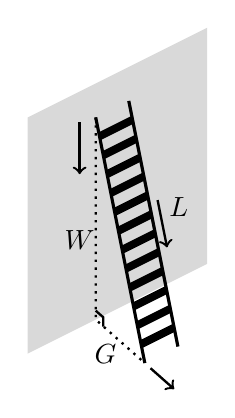
\begin{tikzpicture}[scale=0.6]
	% Wall
	\draw[draw=none,fill=gray!30] (0,0) -- (0,5) -- (3.8,6.9) -- (3.8,1.9) -- (0,0);
	\draw[line width=0.03cm] (2.4,0.2) -- (3.1,0.55);
	% Ladder
	\foreach \x in {0,1,...,11}
		{
		\draw[line width=0.1cm] (2.4 - 0.08*\x,0.2 + 0.4*\x) -- (3.1 - 0.08*\x,0.55 + 0.4*\x);
		};
	\draw[line width=0.04cm] (2.48,-0.2) -- (1.44,5);
	\draw[line width=0.04cm] (3.18,0.15) -- (2.14,5.35);
	% Lines
	\draw[line width=0.03cm,dotted] (1.44,5) -- (1.44,0.72) -- (2.48,-0.2);
	\draw[line width=0.03cm] (1.44,0.91) -- (1.6,0.77) -- (1.6,0.57);
	\draw[line width=0.03cm,->] (1.1,4.9) -- (1.1,3.8);
	\draw[line width=0.03cm,->] (2.6,-0.308) -- (3.1,-0.75);
	
	\draw[line width=0.03cm,->] (2.75,3.25) -- (2.95,2.25);
	% Labels
	\node at (1.65,0) {$G$};
	\node at (1.1,2.4) {$W$};
	\node at (3.2,3.1) {$L$};
	\end{tikzpicture}
	\]
We know that $W^ 2+ G^2= L^2$. When the ladder is $L= 15$~ft extended and is $12$~ft up the wall, we know that\dots
	\[
	\begin{gathered}
	W^2 + G^2= L^2 \\
	9^2 + G^2= 15^2 \\
	81 + G^2= 225 \\
	G^2= 144 \\
	G= 12
	\end{gathered}
	\]
We know that the ladder is sliding down the wall at $3$~ft per second, i.e. $\frac{dW}{dt}= -3$. Also, we know that the ladder is collapsing at $2$~ft per second, i.e. $\frac{dL}{dt}= - 2$. But then\dots
	\[
	\begin{gathered}
	W^ 2+ G^2= L^2 \\
	\dfrac{d}{dt} \left( W^ 2+ G^2 \right)= \dfrac{d}{dt} \, L^2 \\
	2W\, \dfrac{dW}{dt} + 2G\, \dfrac{dG}{dt}= 2L\, \dfrac{dL}{dt} \\
	W\, \dfrac{dW}{dt} + G\, \dfrac{dG}{dt}= L\, \dfrac{dL}{dt} \\
	9(-3) + 12 \, \dfrac{dG}{dt}= 15 (-2) \\
	-27 + 12 \, \dfrac{dG}{dt}= -30 \\
	9 \, \dfrac{dG}{dt}= -3 \\
	\dfrac{dG}{dt}= -\dfrac{1}{3}
	\end{gathered}
	\]
Therefore, the base of the ladder is sliding away from the wall at $-\frac{1}{3} \approx -0.333$~ft per second, i.e. -4~in per second.
}



% Question 6
\newpage
\question[16] Showing all your work, complete the following parts:
	\begin{enumerate}[(a)]
	\item Find the linearization of $f(x)= \sqrt[4]{x}$ at $x= 16$. \pspace
	
		{\itshape We can see that\dots
		\[
		\begin{aligned}
		f(x)&= \sqrt[4]{x}= x^{1/4} \\[0.3cm]
		f'(x)&= \dfrac{1}{4}\, x^{-3/4}= \dfrac{1}{4} \cdot \dfrac{1}{x^{3/4}}= \dfrac{1}{4 \sqrt[4]{x^3}}= \dfrac{1}{4 (\sqrt[4]{x})^3}
		\end{aligned}
		\]
	But then we have\dots
		\[
		\begin{aligned}
		f(16)&=\sqrt[4]{16}= 2 \\[0.3cm]
		f'(16)&= \dfrac{1}{4(\sqrt[4]{16})^3}= \dfrac{1}{4(2^3)}= \dfrac{1}{4(8)}= \dfrac{1}{32}
		\end{aligned}
		\] \par\vspace{0.5cm}
	Therefore, the linearization of $f(x)$ at $x= 8$ is\dots \par\vspace{0.1cm}
		\[
		\ell(x)= y_0 + m(x - x_0)= 2 + \dfrac{1}{32} \, (x - 16) 
		\]
	} \par\vspace{2.6cm}

	\item Use your answer in (a) to approximate $\sqrt[4]{40}$. Express your answer as a decimal. \pspace
	
	{\itshape We have\dots
		\[
		\sqrt[4]{40}= f(40) \approx \ell(40)= 2 + \dfrac{1}{32} \,(40 - 16)= 2 + \dfrac{1}{32} \cdot 24= 2 + \dfrac{3}{4}= 2 + 0.75= 2.75
		\]
	} \vfill
	
	{\itshape\footnotesize Note. In fact, $\sqrt[4]{40} \approx 2.51487$. This means we have approximated $\sqrt[4]{40}$ with only a 9.35\% error!}
	\end{enumerate}

\end{questions}
\end{document}